%%%%%%%%%%%%%%%%%%%%%%%%%%%%%%%%%%%%%%%%%%%%%%%%%%%%%%%%%%%%%%%%%%%%%%%
%%%%%%%%%%%%%%%%%%%%%%%%%%%%%%%%%%%%%%%%%%%%%%%%%%%%%%%%%%%%%%%%%%%%%%%
%%%%%                                                                 %
%%%%%     <file_name>.tex                                             %
%%%%%                                                                 %
%%%%% Author:      <author>                                           %
%%%%% Created:     <date>                                             %
%%%%% Description: <description>                                      %
%%%%%                                                                 %
%%%%%%%%%%%%%%%%%%%%%%%%%%%%%%%%%%%%%%%%%%%%%%%%%%%%%%%%%%%%%%%%%%%%%%%
%%%%%%%%%%%%%%%%%%%%%%%%%%%%%%%%%%%%%%%%%%%%%%%%%%%%%%%%%%%%%%%%%%%%%%%

\chapter{Specification}

\todo{Diagram with all sensors etc.}

\section{Sensors}

\subsection{Laser Distance Sensors}

In total four laser distance sensors were used to assess the vehicle attitude in relation to the rail.

Two high precision sensors were employed to measure the lateral alignment to the track at the front and the back of the pod. These sensors provided the input for the yaw controller in order to actively ensure that the pod is correctly aligned with the track and not exercising an torque on the rail.

Two smaller form-factor sensors were also installed at the front and back of the pod to measure the pods vertical alignment. These were mostly used to asses the performance of the clamping system.

\subsection{Pressure Sensors}

\subsubsection{Ambient pressure sensors}

A high-precision pressure sensor was installed to monitor the ambient pressure. Two further ambient pressure sensors were installed inside of each high-voltage battery pack, as these were pressurized. If the pressure inside the battery packs drops too low the battery cells could be permanently damage. Therefore, it was necessary to monitor these values and re-pressurize the pod's environment in the event of a leak.

\subsubsection{Braking pressure sensors}

Four high-pressure sensors were installed in the braking system. One in each braking piston to measure the pressure with which the brakes actuate and to determine their status. Additionally, one sensor was installed in each reservoir holding the pressure used to engage the brakes in order to monitor brake health. The braking system consisted of two independent hydraulic systems for redundancy, thus two sets of sensors were necessary.

\subsection{Navigational Sensors}

Two laser contrast sensors were used to detect optical marking on the wall of the test tube. The optical markings occur in intervals of 30m and can therefore be used to determine the location of the pod along the tube and calculate it's velocity.

\section{Propulsion system}

Four two-phase electric motors are used to accelerate the pod. Each is driven by a separate inverter. The inverters are controlled via a CAN bus and two digital safety signals. The RFE signal enables the inverter and the RUN signal connects the high voltage from the battery to the motor. The inverter can be configured over the CAN bus. Subsequently, both torque and speed commands can be given to the inverters to drive the motors. Furthermore, the inverters provide telemetry over CAN including the following:

\begin{itemize}
    \item Inverter status
    \item DC bus voltage
    \item DC current
    \item Motor RPMs
    \item Motor RMS current
    \item Inverter temperature
    \item Motor temperature
\end{itemize}

\section{Battery Management System (BMS)}

Two battery management modules (one in each battery pack) are responsible for balancing the battery cells and monitoring them. These modules are also connected to a CAN bus and provide the following telemetry over it:

\begin{itemize}
    \item High-voltage isolation status
    \item Battery Pack Voltage
    \item Discharge/Charge current
    \item Lowest cell voltage
    \item Highest cell temperature
\end{itemize}

\section{Telemetry and Control Panel}

To monitor the pod a network is made available inside the tube. The pod connects to this network and must transmit all telemetry necessary to assess the pod's state and make sure it is safe. In addition, the pod is controlled over the network. Should the connection to the pod fail at any point, the pod must enter a safe state immediately. To control the pod and display telemetry a control panel application was developed.

\begin{figure}[H]
  \centering 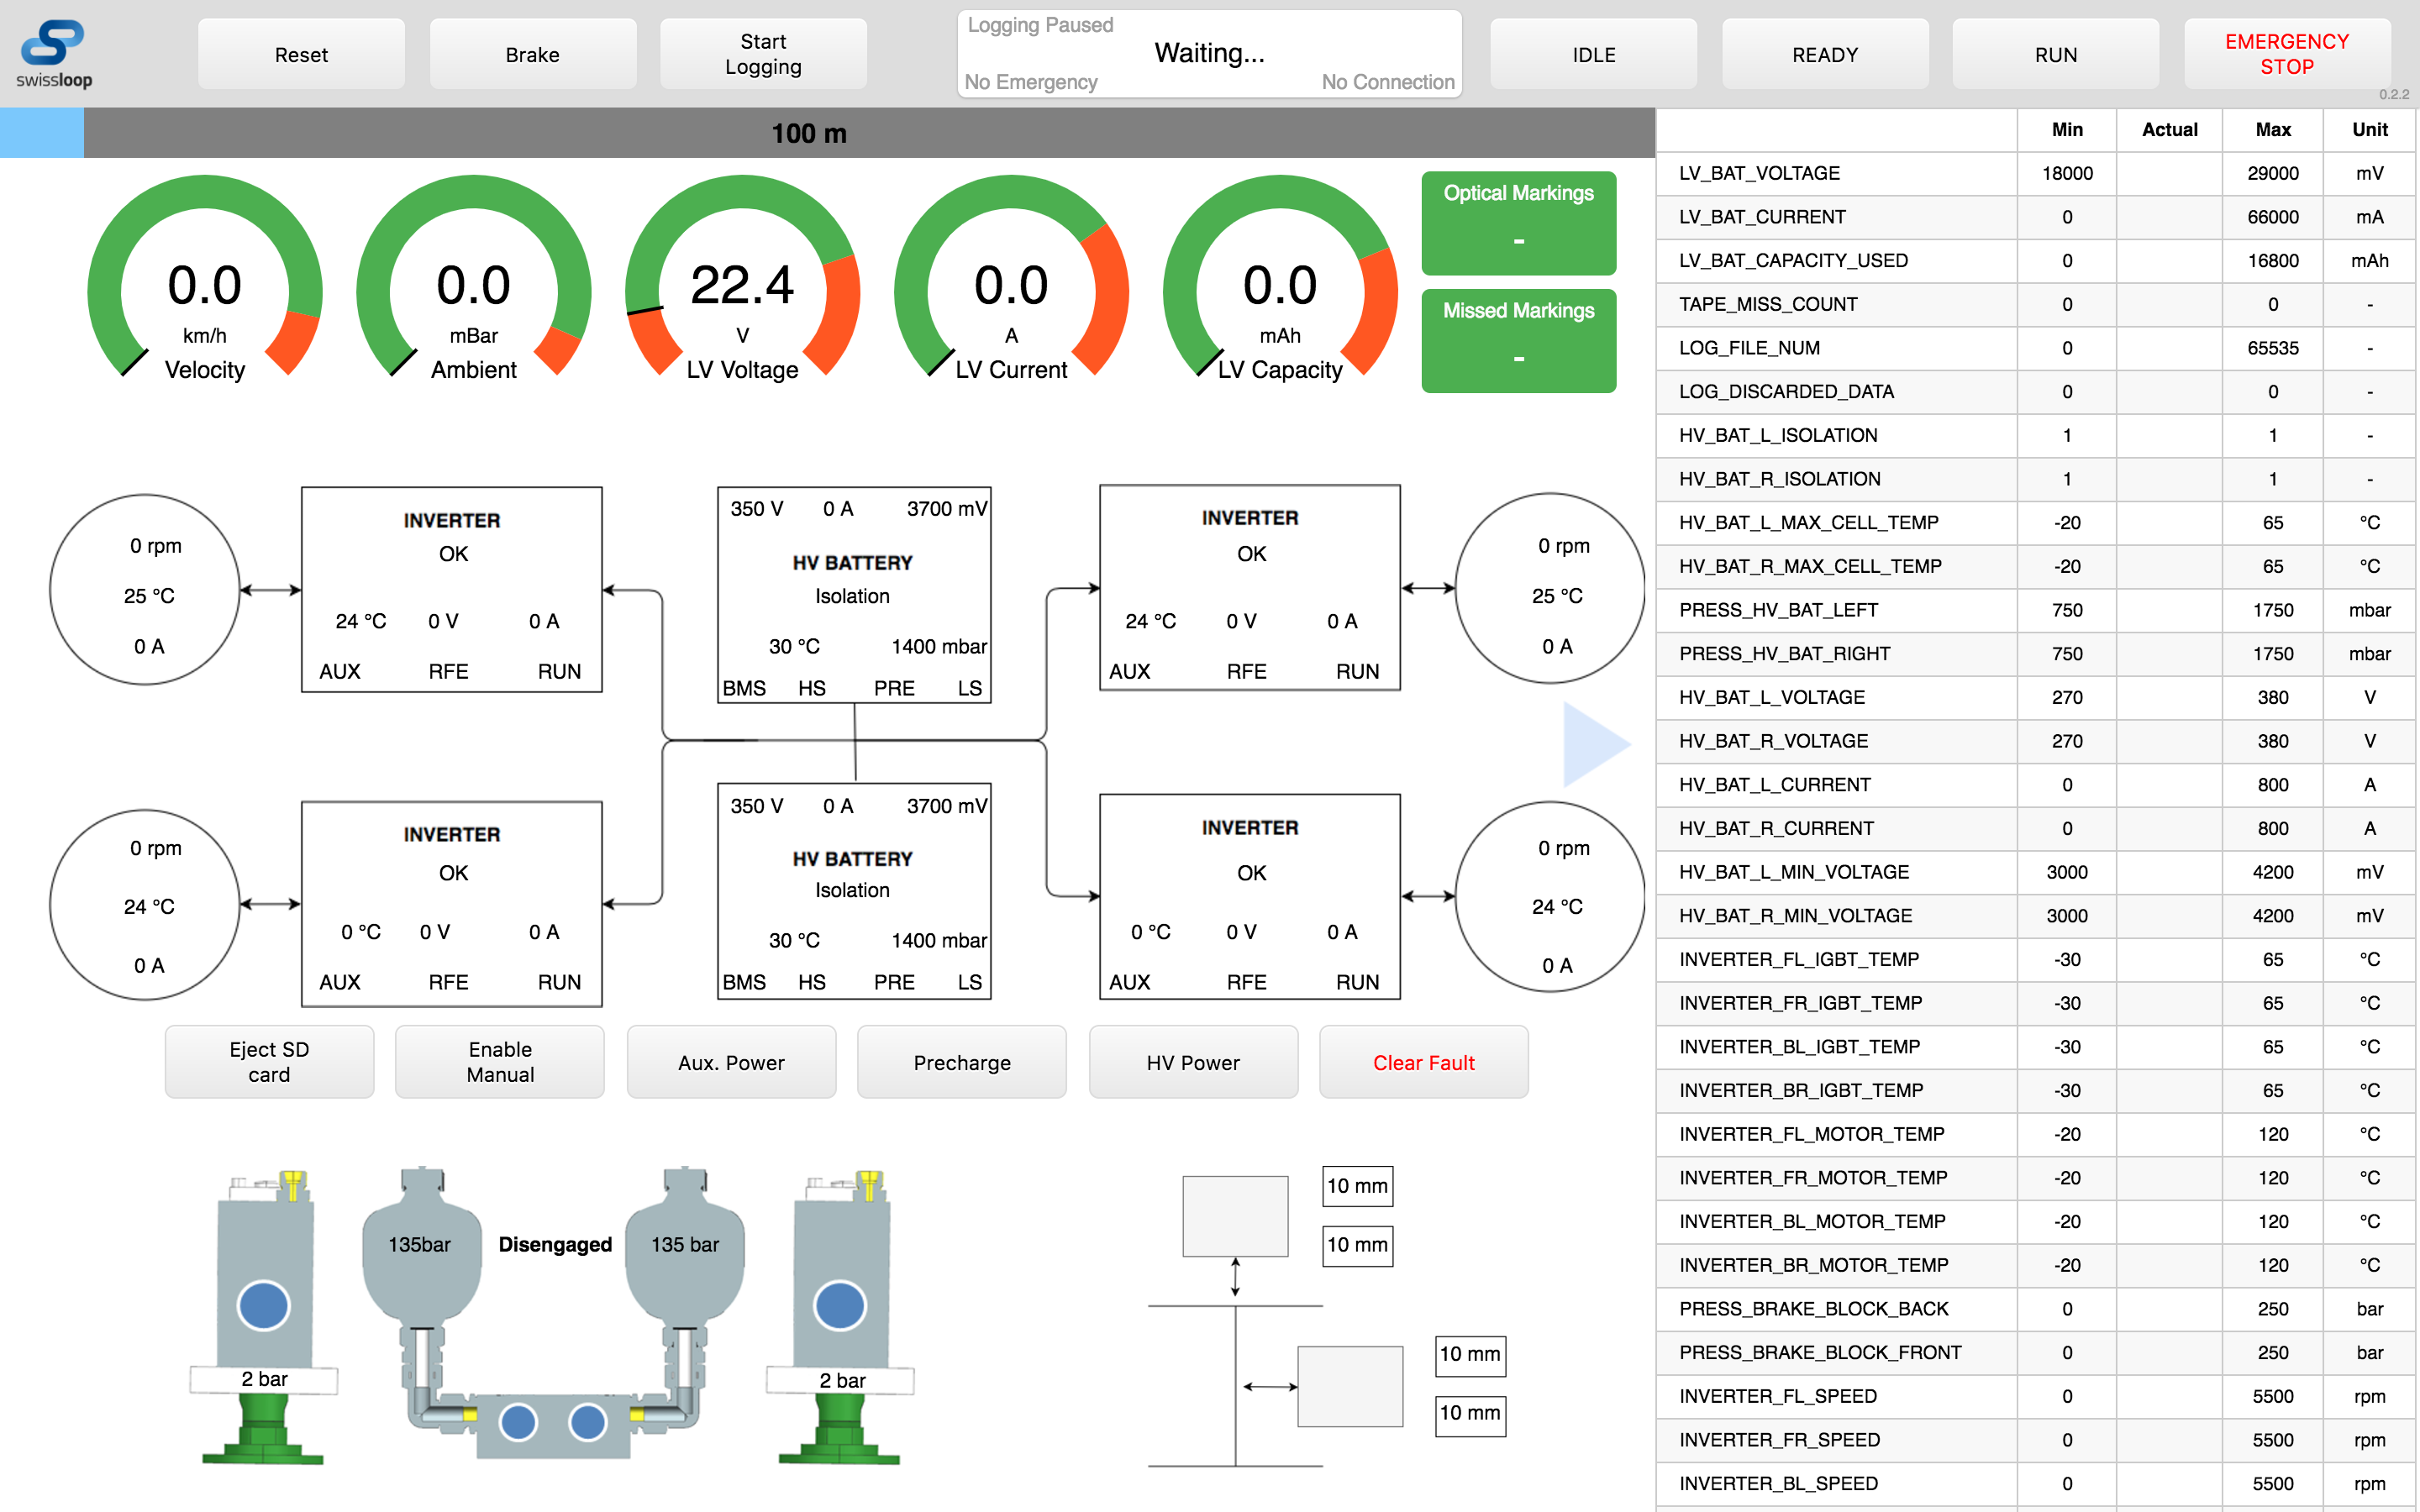
\includegraphics[width=1.0\textwidth]{./figures/Screen_Shot_Control_Panel.png}
  \caption{Screen shot of the control panel.}
\end{figure}

\section{Data Logging}

In order to verify the pod's performance and diagnose possible failures, we wanted to be able to log as much data as possible. Therefore, we set a goal to log all sensor data that comes into the system.

\todo{Maybe add screenshot of plotting software?}

\section{Control and State Machine}

Overall, the pod is controlled by a finite state machine (FSM). The FSM must incorporate all critical safety checks and is also used to allow the pod to complete the run autonomously. In order to improve testability, the FSM should have the minimum number of states necessary for the desired functionality. To this end we also decided to minimize the number of automatic state transitions, minimizing the risk of bugs in the implementation.

\section{Correctness and Testability}

The highest priority for this system was to ensure correctness and safety. Therefore it was important to minimize sources of errors and implement the system with testability in mind. Tests include unit tests for individual control sequences and algorithms, as well as functional tests.


%%% Local Variables: 
%%% mode: latex
%%% TeX-master: "../report_template"
%%% End: 
